\documentclass{article}
\usepackage[margin=1in]{geometry}
\usepackage{amsmath, amsthm, amssymb}
\usepackage{physics}
\usepackage{float}
\usepackage{graphicx}
\usepackage{subcaption}
\usepackage{hyperref}

\DeclareMathOperator{\sinc}{sinc}

\title{Magnetic Nozzle Eigenvalue Problem Results}
\author{Hunt Feng}
\date{\today}

\begin{document}
\maketitle

\section{Exact Solution}
In this document, I will list all the methods I tried and their results for the eigenvalue problem
\begin{equation}
    \omega^2\tilde{v} + 2iv_0\omega\pdv{\tilde{v}}{z} + (1-v_0^2)\pdv[2]{\tilde{v}}{z} = 0, \tilde{v}(-1)=\tilde{v}(1) = 0
    \label{eq:original-problem}
\end{equation}
where $v_0\in\mathbb{R}$ is a constant. In thsi problem, we need to solve for eigenvalues $\omega$ and their corresponding eigenfunctions $\tilde{v}$.
\begin{equation}
    \tilde{v} = \exp(-\frac{i\omega}{v_0+1})\left[ \exp(i\omega\frac{z+1}{v_0+1}) - \exp(i\omega\frac{z+1}{v_0-1}) \right] \text{ where } \omega=\frac{n\pi(1-v_0^2)}{2}
\end{equation}
All eigenvalues are real, so all modes are stable.
\begin{figure}[H]
    \centering
    \begin{subfigure}[b]{0.45\linewidth}
        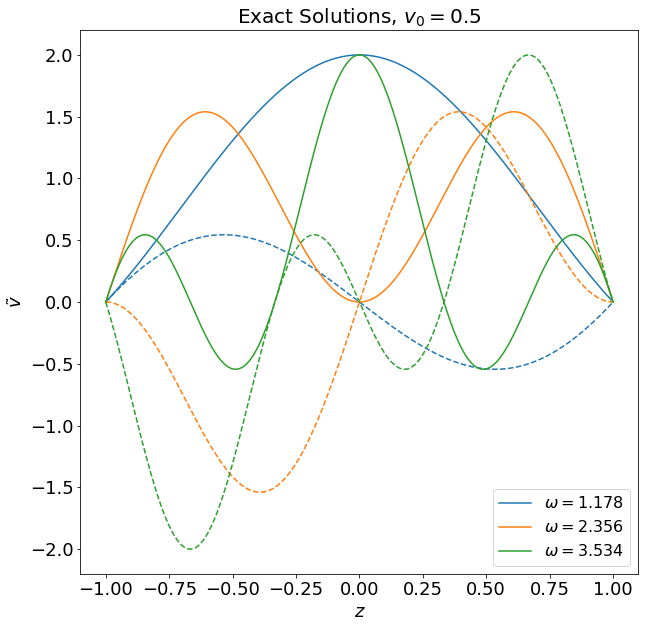
\includegraphics[width=\linewidth]{img/eigenfunctions-exact-v0=0.5.png}
        \caption{}
    \end{subfigure}%
    \begin{subfigure}[b]{0.45\linewidth}
        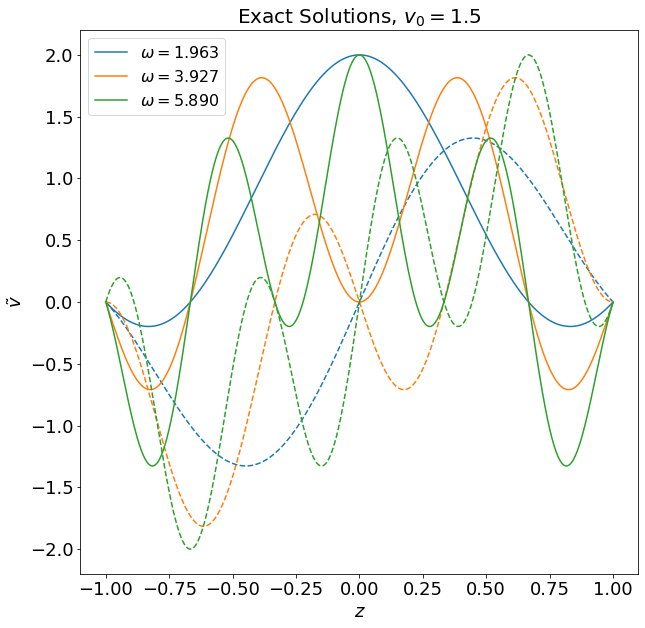
\includegraphics[width=\linewidth]{img/eigenfunctions-exact-v0=1.5.png}
        \caption{}
    \end{subfigure}
    \caption{First few exact eigenfunctions(ground mode, $\omega=0$, not included).}
    \label{fig:eigenvectors-constant-v}
\end{figure}

\newpage
\section{Finite Element}
Assume $\tilde{v}(z) = \sum_{j} c_ju_j(z)$, where $u_j(z)$ are basis functions. Left multiply $u_i(z)$ on both sides of the equation, then take the inner product,

$$ \sum_{j} \left[ \omega^2 (u_i,u_j)  + 2i\omega v_0 (u_i,u_j') + (1-v_0^2)(u_i,u_j'') \right]c_j = 0 $$
where $(\cdot,\cdot)$ denotes the inner product.

Let $A_2=(u_i,u_j)$, $A_1=2iv_0(u_i,u_j')$, and $A_0=(1-v_0^2)(u_i,u_j'')$. Denote $\mathbf{c} = [c_j]^T$. We have a polynomial eigenvalue problem
$$ (\omega^2 A_2 + \omega A_1 + A_0)\mathbf{c} = \mathbf{0} $$

If $u_j(z)$ are orthonormal functions on $[-1,1]$, then the polynomial eigenvalue problem can be written as an algebraic eigenvalue problem
$$ 
\mqty[ O & I \\ A_{21} & A_{22} ]\mqty[\mathbf{c} \\ \omega\mathbf{c}]
= \omega\mqty[\mathbf{c} \\ \omega\mathbf{c}]
$$
where $O$ is $N\times N$ zero matrix, $I$ is $N\times N$ identity matrix, and
$$ A_{21} = (1-v_0^2)(u_i',u_j'),\;\;\; A_{22} = -2iv_0(u_i,u_j') $$

\subsection{DVR methods}
Let $u_j(z)$ be basis functions that satisfy the boundary condition $u_j(-1)=u_j(1)=0$, and the Kronecker delta property
$$ u_j(z_k) = \delta_{jk} $$
By using Gaussian quadrature with quadrature nodes $z_k\in[-1,1]$, we see that $u_i(z)$ are othornormal on $[-1,1]$ if we scale them correctly,
$$ \int_{-1}^{1} u_i(z)u_j(z) = \sum_{k} w_ku_i(z_k)u_j(z_k) = \delta_{ij} $$



\subsubsection{Sine DVR}
Let $\psi_n(z) = \sin(\frac{n\pi}{2}(z+1)), n=1,\cdots,N$ be the orthorgonal functions on $[-1,1]$, and define the DVR basis functions by
$$ u_j(z) = w_j\sum_{n=1}^N \psi_n(z)\psi_n^*(z_j) $$

\begin{figure}[H]
    \centering
    \begin{subfigure}[b]{0.45\linewidth}
        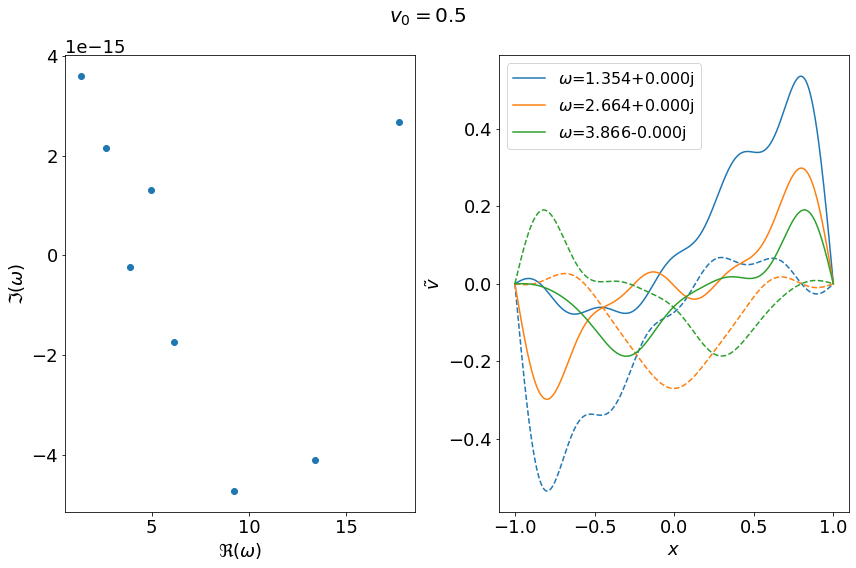
\includegraphics[width=\linewidth]{img/results-sine-dvr-N=9,v0=0.5.png}
        \caption{}
    \end{subfigure}%
    \begin{subfigure}[b]{0.45\linewidth}
        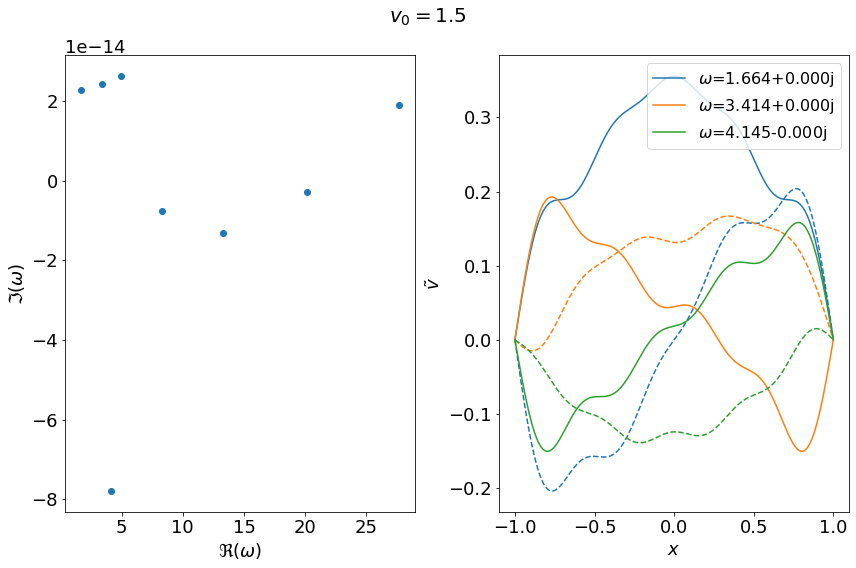
\includegraphics[width=\linewidth]{img/results-sine-dvr-N=9,v0=1.5.png}
        \caption{}
    \end{subfigure}
    \caption{Using $N=9$ basis functions. All modes are stable.}
    \label{fig:results-sine-dvr}
\end{figure}
This looks hopeful! However, when we increase velocity, $v_0$, or the number of basis function, $N$. Unstable modes occur in supersonic case,

\begin{figure}[H]
    \centering
    \begin{subfigure}[b]{0.45\linewidth}
        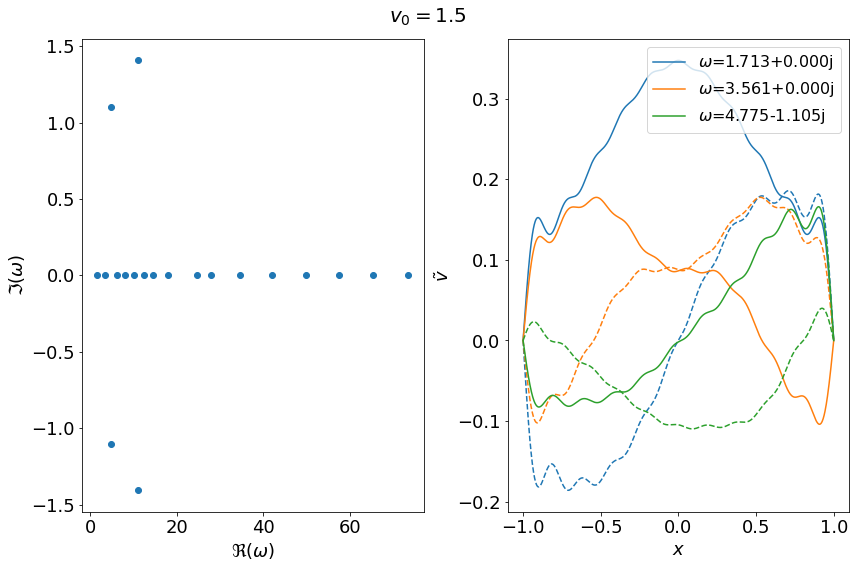
\includegraphics[width=\linewidth]{img/results-sine-dvr-N=21,v0=1.5.png}
        \caption{Using $N=21$ basis function.}
    \end{subfigure}%
    \begin{subfigure}[b]{0.45\linewidth}
        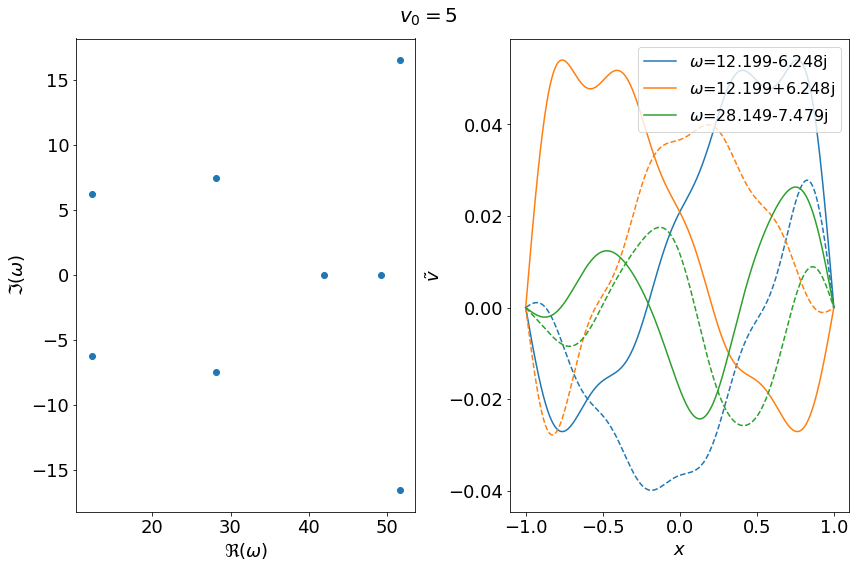
\includegraphics[width=\linewidth]{img/results-sine-dvr-N=9,v0=5.png}
        \caption{Using $N=9$ basis function.}
    \end{subfigure}
    \caption{Increasing $N$ or $v_0$, things become more unstable in supersonic case.}
    \label{fig:results-sine-dvr-unstable}
\end{figure}


\subsubsection{Sinc DVR}
Using the normalized $\sinc(x)=\sin(\pi x)/(\pi x)$, the basis functions are 
$$u_j(z) = \frac{\sinc((z-z_j)/\Delta z)}{\sqrt{\Delta z}}$$
where $z_j\in[-1,1]$ are the quadrature nodes.
\begin{figure}[H]
    \centering
    \begin{subfigure}[b]{0.45\linewidth}
        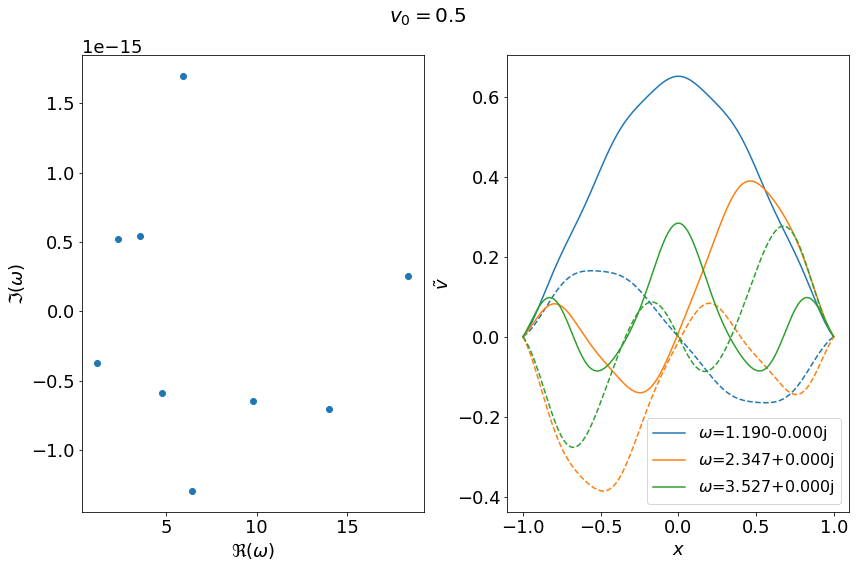
\includegraphics[width=\linewidth]{img/results-sinc-dvr-dx=0.2,v0=0.5.png}
        \caption{Using $\Delta x=0.2$.}
    \end{subfigure}%
    \begin{subfigure}[b]{0.45\linewidth}
        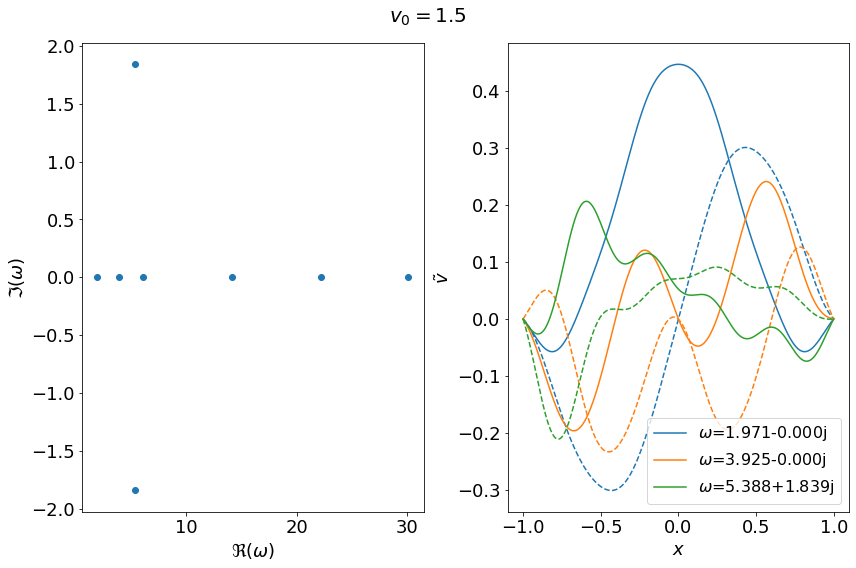
\includegraphics[width=\linewidth]{img/results-sinc-dvr-dx=0.2,v0=1.5.png}
        \caption{Using $\Delta x=0.2$.}
    \end{subfigure}
    \caption{No matter what $\Delta x$ I use, there will be unstable modes in supersonic case.}
    \label{fig:results-sinc-dvr}
\end{figure}

\begin{figure}[H]
    \centering
    \begin{subfigure}[b]{0.45\linewidth}
        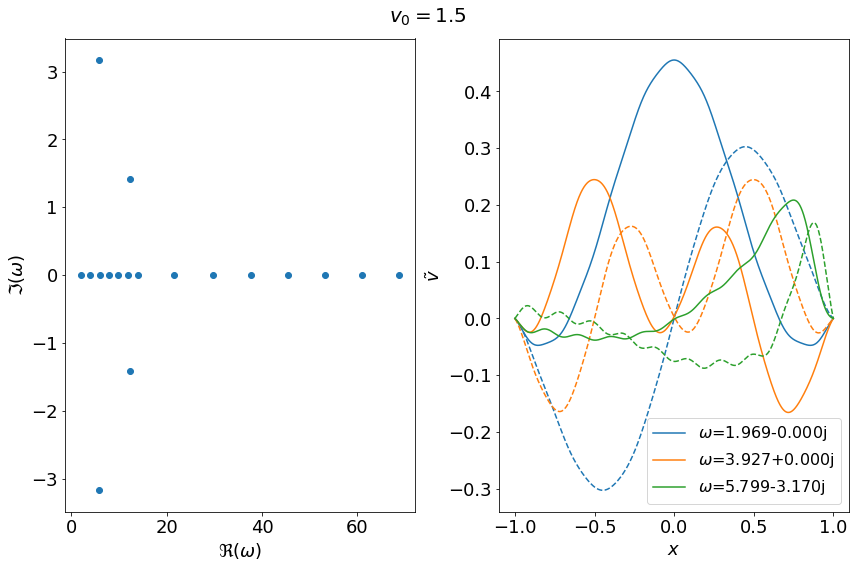
\includegraphics[width=\linewidth]{img/results-sinc-dvr-dx=0.1,v0=1.5.png}
        \caption{Using $\Delta x=0.1$}
    \end{subfigure}%
    \begin{subfigure}[b]{0.45\linewidth}
        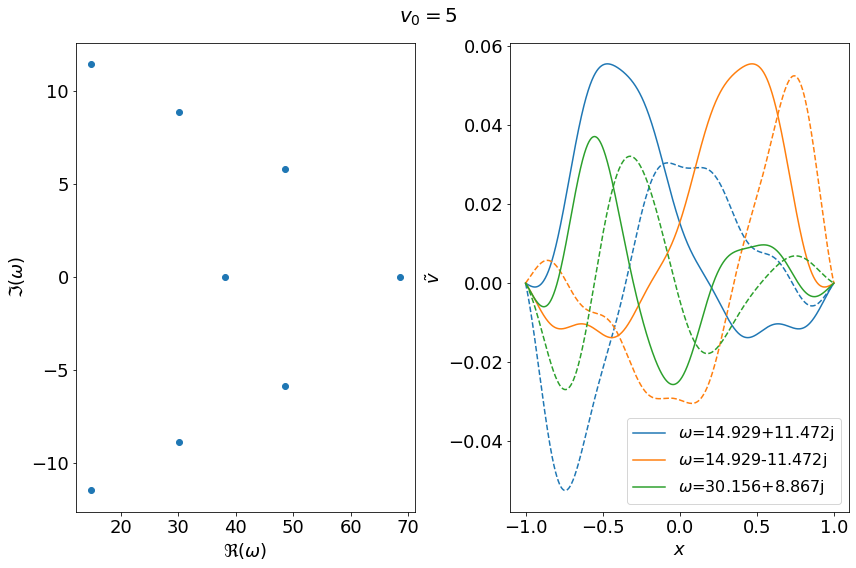
\includegraphics[width=\linewidth]{img/results-sinc-dvr-dx=0.2,v0=5.png}
        \caption{Using $\Delta x=0.2$.}
    \end{subfigure}
    \caption{Decreasing $\Delta x$ (equivalent to increasing number of basis functions) or increasing $v_0$, things become more unstable in supersonic case.}
    \label{fig:results-sinc-dvr-unstable}
\end{figure}

Similar to Sine DVR, if we decrease the $\Delta z$ (equivalent to increasing number of basis functions), or increase $v_0$. Modes become unstable in supersonic case. 


\subsection{Non-DVR methods}
\subsubsection{Linear Element}
Let $ \tilde{v}(z) = \sum_{j=1}^{N} c_ju_j(z) $ where $u_j(z)$ are tent functions that peaks at $x_j\in(-1,1)$.
\begin{figure}[H]
    \centering
    \begin{subfigure}[b]{0.45\linewidth}
        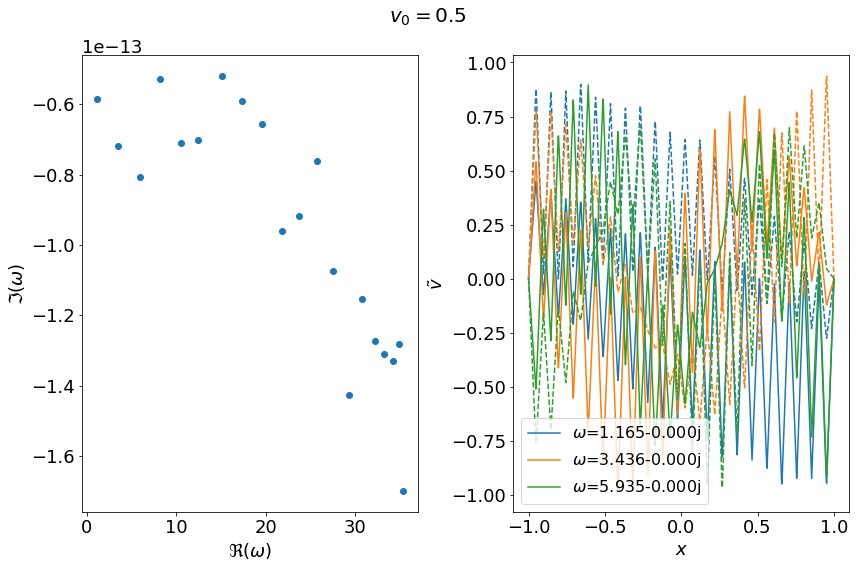
\includegraphics[width=\linewidth]{img/results-linear-N=40,v0=0.5.png}
        \caption{All modes are stable.}
    \end{subfigure}%
    \begin{subfigure}[b]{0.45\linewidth}
        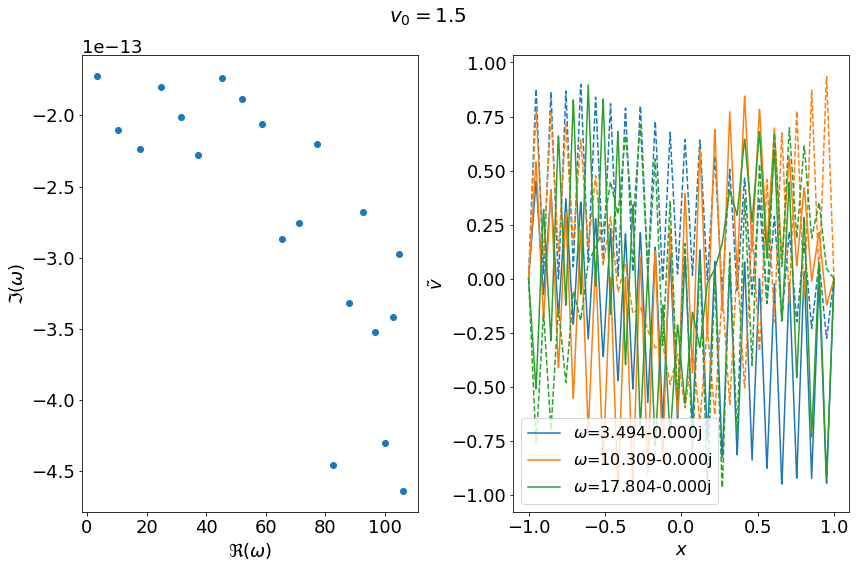
\includegraphics[width=\linewidth]{img/results-linear-N=40,v0=1.5.png}
        \caption{Some modes are unstable.}
    \end{subfigure}
    \caption{Using $N=40$, all modes are stable.}
    \label{fig:results-linear}
\end{figure}

\begin{figure}[H]
    \centering
    \begin{subfigure}[b]{0.45\linewidth}
        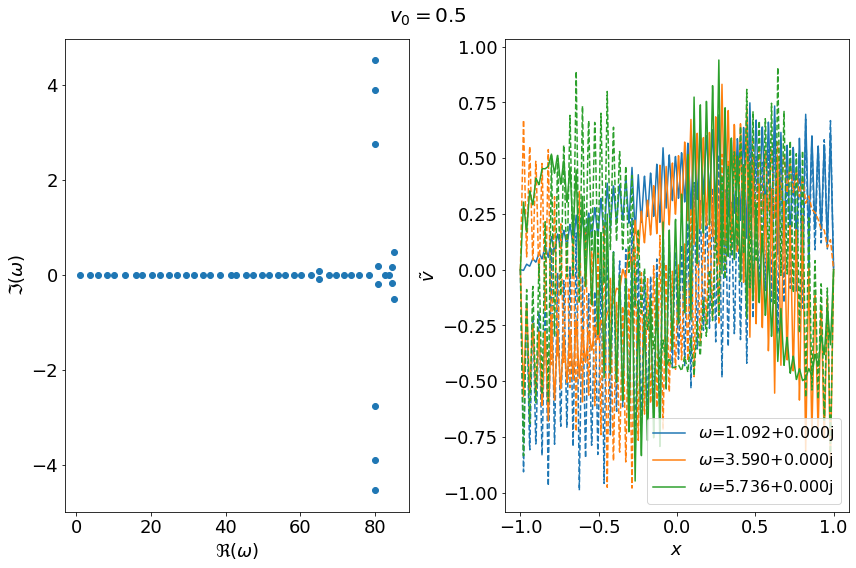
\includegraphics[width=\linewidth]{img/results-linear-N=100,v0=0.5.png}
        \caption{Using $N=100$. This time unstable modes even occur in subsonic case.}
    \end{subfigure}%
    \begin{subfigure}[b]{0.45\linewidth}
        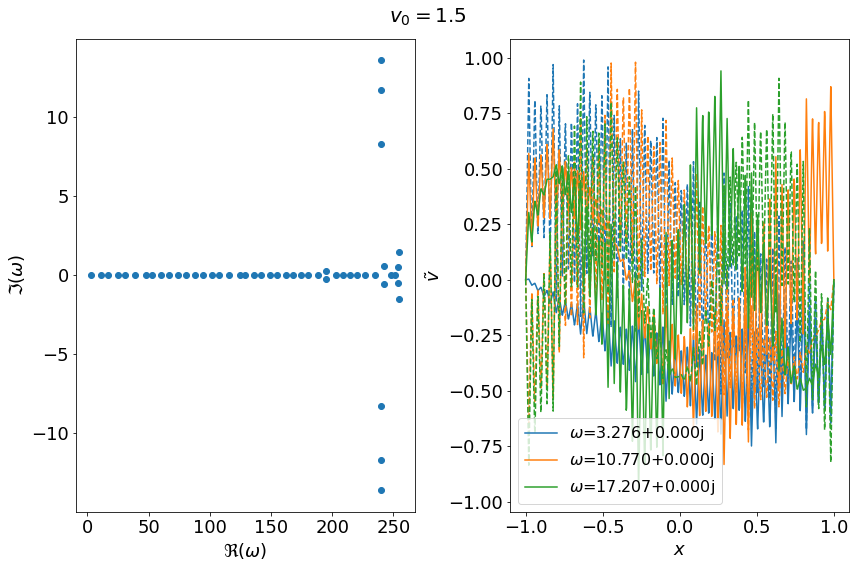
\includegraphics[width=\linewidth]{img/results-linear-N=100,v0=1.5.png}
        \caption{Using $N=100$.}
    \end{subfigure}
    \caption{Increasing $N$, things become more unstable in supersonic case. Increasing $v_0$ will increase the magnitude of growth rate of the modes, but the effect is not significant.}
    \label{fig:results-linear-unstable}
\end{figure}

\subsubsection{Sine}
Let $ \tilde{v}(z) = \sum_{j=1}^{N} c_ju_j(z) $ where $u_j(z)=\sin(\frac{n\pi}{2}(z+1))$.
\begin{figure}[H]
    \centering
    \begin{subfigure}[b]{0.45\linewidth}
        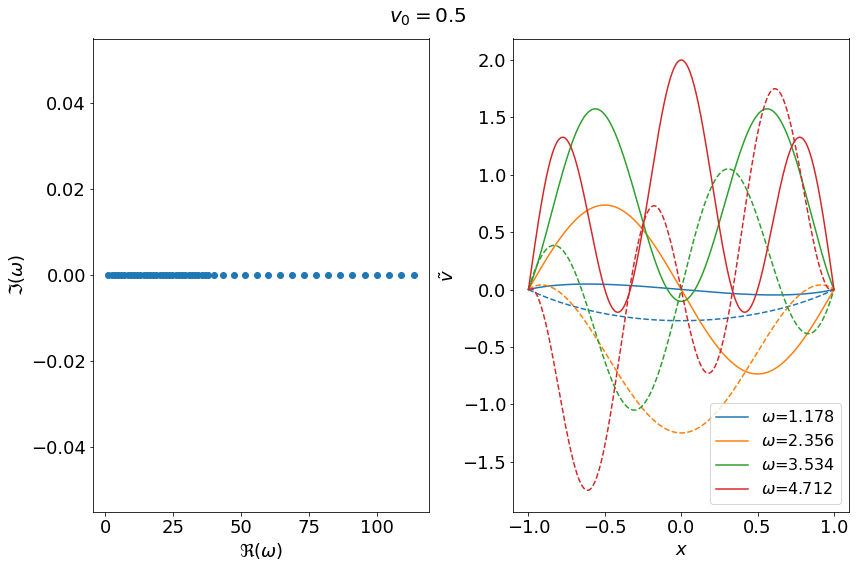
\includegraphics[width=\linewidth]{img/results-sine-N=50,v0=0.5.png}
        \caption{Using $N=50$.}
    \end{subfigure}%
    \begin{subfigure}[b]{0.45\linewidth}
        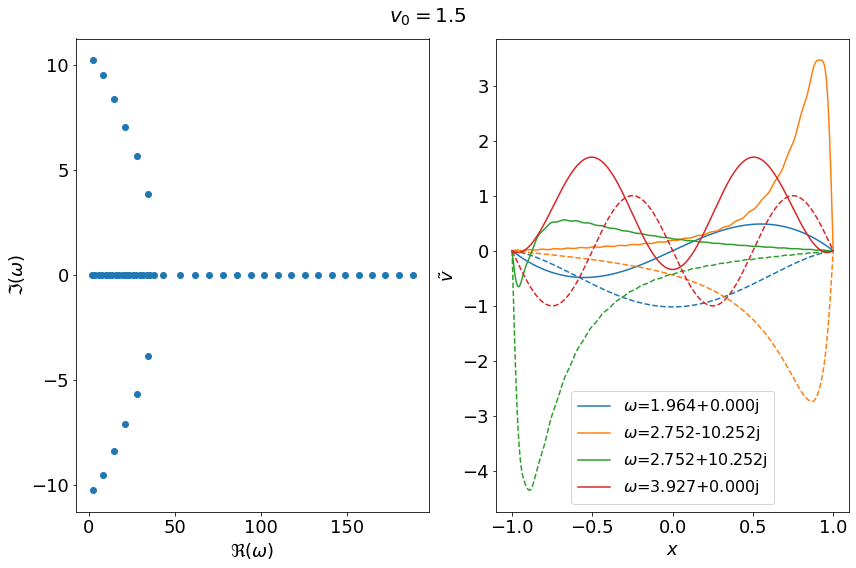
\includegraphics[width=\linewidth]{img/results-sine-N=50,v0=1.5.png}
        \caption{Using $N=50$.}
    \end{subfigure}
    \caption{Unstable modes in supersonic case.}
    \label{fig:results-sine}
\end{figure}

\begin{figure}[H]
    \centering
    \begin{subfigure}[b]{0.45\linewidth}
        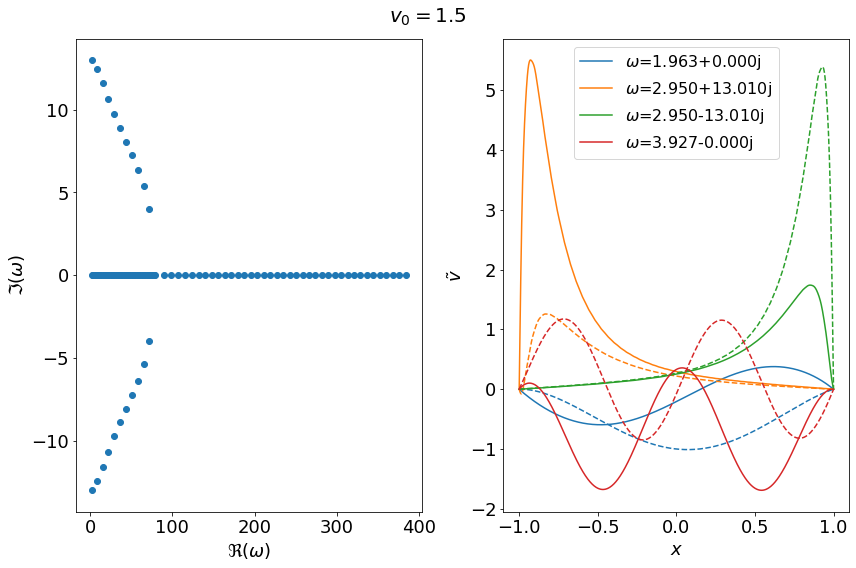
\includegraphics[width=\linewidth]{img/results-sine-N=100,v0=1.5.png}
        \caption{Using $N=50$.}
    \end{subfigure}%
    \begin{subfigure}[b]{0.45\linewidth}
        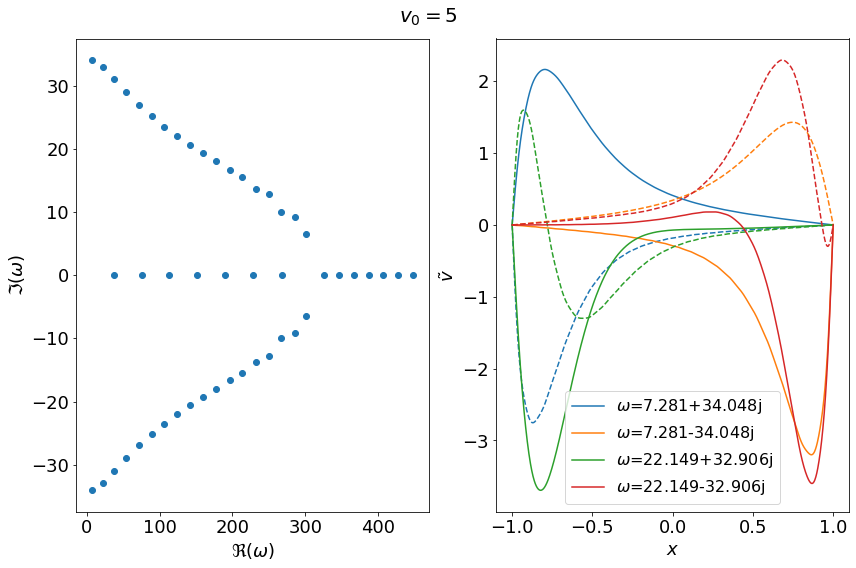
\includegraphics[width=\linewidth]{img/results-sine-N=50,v0=5.png}
        \caption{Using $N=50$.}
    \end{subfigure}
    \caption{Increasing $N$ or $v_0$ makes things more unstable in supersonic case.}
    \label{fig:results-sine-unstable}
\end{figure}


\newpage
\section{Finite Difference}
Expressing the differentiation operator as matrices, we have
$$ (\omega^2 A_2 + \omega A_1 + A_0)\mathbf{\tilde{v}} = \mathbf{0} $$
where $A_2 = I$, $A_1 = 2iv_0\pdv*{z}$, and $(1-v_0^2)\pdv*[2]{z}$. Lastly, $\mathbf{\tilde{v}} = [\tilde{v}_j]^T$ is the value of $\tilde{v}$ at each grid point $x_j\in[-1,1]$.

\begin{figure}[H]
    \centering
    \begin{subfigure}[b]{0.45\linewidth}
        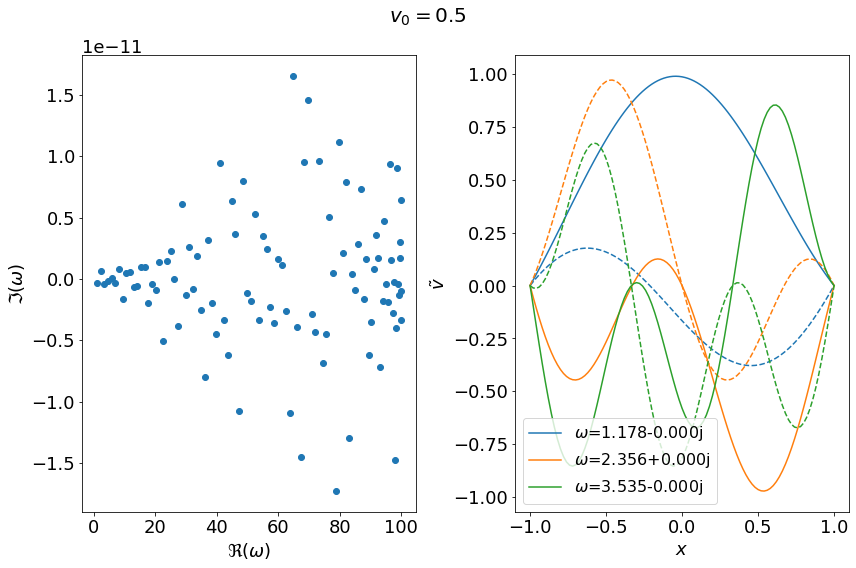
\includegraphics[width=\linewidth]{img/results-fd-N=101,v0=0.5.png}
        \caption{All modes are stable.}
    \end{subfigure}%
    \begin{subfigure}[b]{0.45\linewidth}
        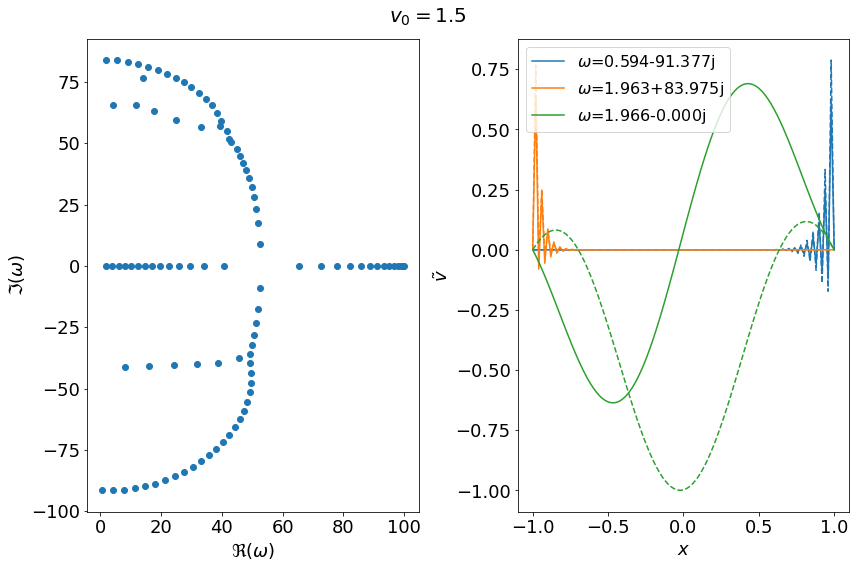
\includegraphics[width=\linewidth]{img/results-fd-N=101,v0=1.5.png}
        \caption{Some modes are unstable.}
    \end{subfigure}
    \caption{Using $\Delta x=0.1$, some modes are unstable in supersonic case. In fact, no matter what $\Delta x$ I use, there will be unstable modes in supersonic case.}
    \label{fig:results-fd}
\end{figure}

\begin{figure}[H]
    \centering
    \begin{subfigure}[b]{0.45\linewidth}
        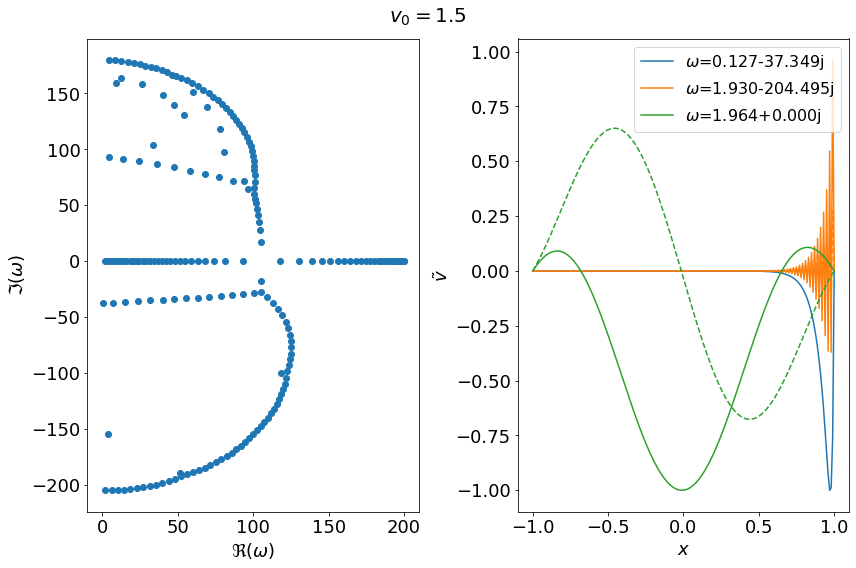
\includegraphics[width=\linewidth]{img/results-fd-N=201,v0=1.5.png}
        \caption{}
    \end{subfigure}%
    \begin{subfigure}[b]{0.45\linewidth}
        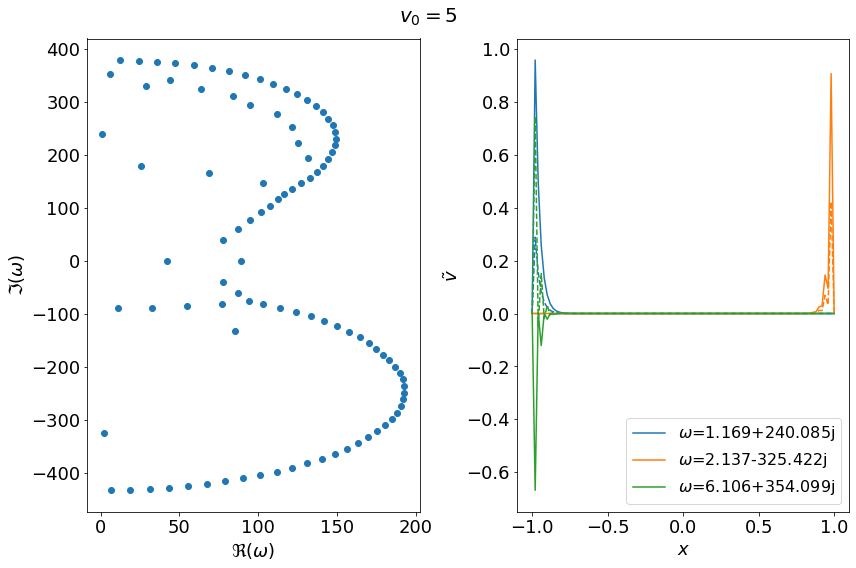
\includegraphics[width=\linewidth]{img/results-fd-N=101,v0=5.png}
        \caption{}
    \end{subfigure}
    \caption{Increasing $N$ or $v_0$ makes the unstable modes more unstable in supersonic case.}
    \label{fig:results-fd-unstable}
\end{figure}

\subsection{Reduction to Normal Form}
The equation 
$$ \omega^2\tilde{v}(z) + 2i\omega\tilde{v}'(z) + (1-v_0^2)\tilde{v}''(z) = 0, \tilde{v}(-1) = \tilde{v}(1) = 0 $$
can be reduced to normal form
$$ u''(z) + r(z)u(z) = 0, u(-1) = u(1) = 0 $$
by doing the following variable change
$$
u(z) = \exp\left(\frac{iv_0\omega}{1-v_0^2}\right)\tilde{v}(z); \;\;\;
r(z) = \frac{\omega^2}{(1-v_0^2)^2}
$$

\begin{figure}[H]
    \centering
    \begin{subfigure}[b]{0.45\linewidth}
        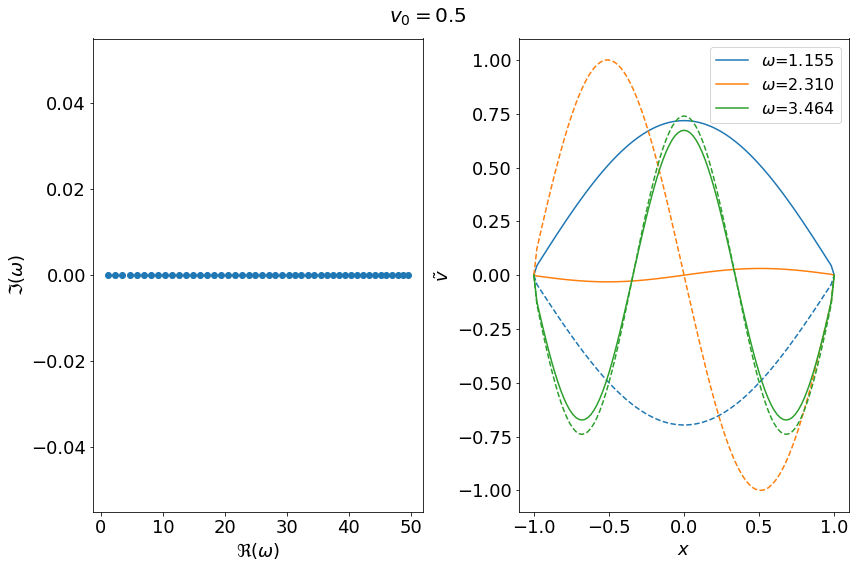
\includegraphics[width=\linewidth]{img/results-normal-v0=0.5.png}
        \caption{}
    \end{subfigure}%
    \begin{subfigure}[b]{0.45\linewidth}
        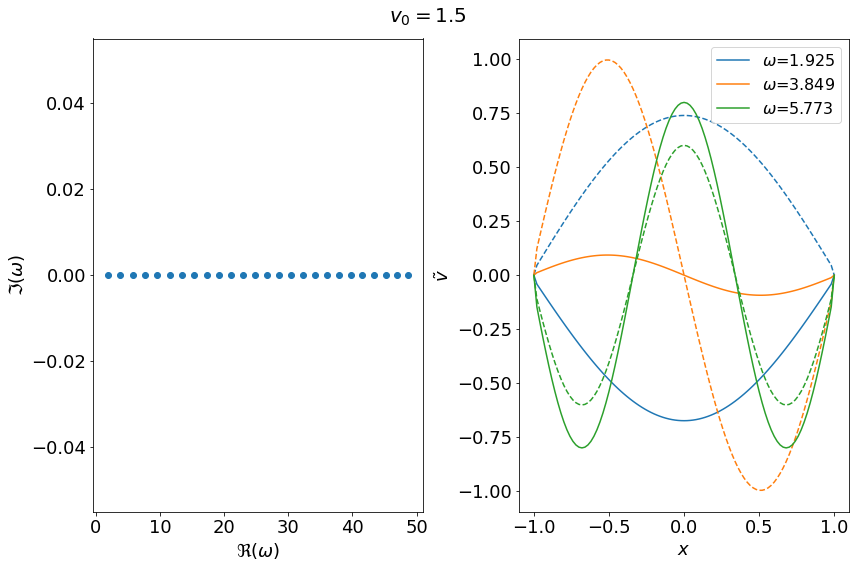
\includegraphics[width=\linewidth]{img/results-normal-v0=1.5.png}
        \caption{}
    \end{subfigure}
    \caption{Finally, all modes are stable.}
    \label{fig:results-normal}
\end{figure}

\end{document}